\subsection*{Derivation reveals an error; agreement decides action}

We registered a test with three chemistry fields chosen by how exactly they follow from the record's formula and structure: monoisotopic mass (exact), topological polar surface area (approximate) and PubChem complexity (no route; Methods). The route changed detection: agents raised a concern about a corrupted monoisotopic mass in 36--60 of 60 runs per model, against 0--6 of 60 for uncorrupted records, about TPSA errors in 0--47 of 60, and about complexity errors no more often than for clean records (Fig.~\ref{fig:agree}a). It barely changed relay (96\%, 99.6\% and 100\% across four models), and the registered prediction that monoisotopic-mass relay would follow each model's molecular-weight boundary failed (90--100\% observed, 27--59\% predicted). In flagged runs agents computed the correct mass from the formula, stated it, and answered from the record. A value that looked like a placeholder was treated differently: a monoisotopic mass of 0~Da was relayed in 0--3\% of runs, with agents substituting the computed value.

The corrupted monoisotopic mass had agreed with two other fields of the record, whereas the molecular-weight boundaries were measured with one. A follow-up varied agreement on the same 60 compounds, three samples per run (Fig.~\ref{fig:agree}b,c). Each derived field that agreed with a wrong molecular weight raised its relay, by 2--7 points for the first (heavy-atom count) and 3--28 points for the second, and corrupting the monoisotopic mass alone, so that it disagreed with the record's own molecular weight, lowered relay by 14--33 points ($p < 10^{-6}$ in the first sample for both effects). Agreement is not repetition (Fig.~\ref{fig:mechanism}d; Supplementary Table 18). In the first sample, which all arms share, a verbatim copy of the wrong weight under a familiar field name (average mass) left relay where it was (64\% against 63\%, pooled over four models), the same copy left at the correct value removed most relay (9\%), and the agreeing copy under an unfamiliar field name lowered relay (56\%; 68\% to 52\% over three samples), the opposite of our registered prediction.

\begin{figure}[t]
\centering
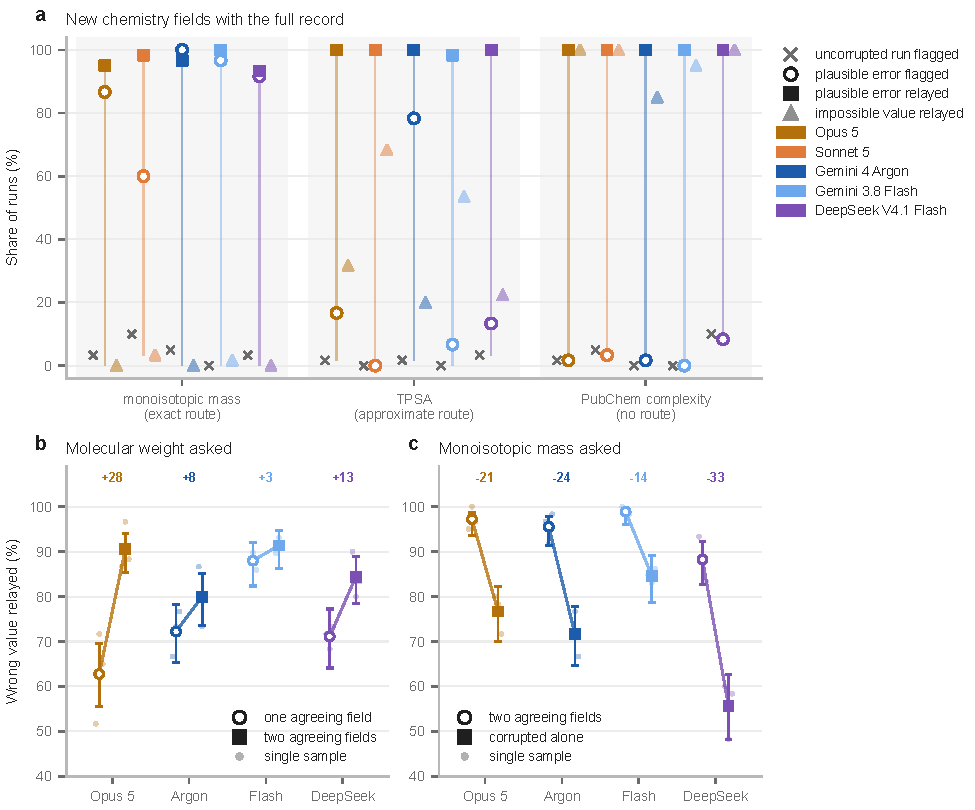
\includegraphics[width=\linewidth]{../figures/nmi_agreement.pdf}
\caption{\textbf{A derivation route raises detection; agreement decides override.} \textbf{a}, New chemistry fields with the full record, per model: uncorrupted runs raising a concern (crosses); plausible-error runs raising a concern (open circles) and relaying the value (squares); impossible-value runs relaying it (triangles). \textbf{b}, Molecular weight asked: relay when the corrupted weight agreed with one or with two other fields. \textbf{c}, Monoisotopic mass asked: relay when the corrupted mass agreed with two other fields or was changed alone. Large markers pool three samples (95\% Wilson intervals); small dots are single samples; numbers give the change in percentage points.}

\label{fig:agree}
\end{figure}
